% Figure from MATH 591 notes, section 66 (Lecture 22).
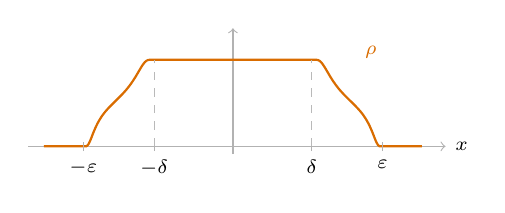
\begin{tikzpicture}[scale=1.0]
\draw[->, gray!60] (-2.6,0) -- (2.7,0) node[right, font=\scriptsize, text=black] {$x$};
\draw[->, gray!60] (0,-0.1) -- (0,1.5);
\draw[orange!85!black, thick] plot[smooth] coordinates {(-2.400,0.000) (-2.380,0.000) (-2.360,0.000) (-2.340,0.000) (-2.320,0.000) (-2.300,0.000) (-2.280,0.000) (-2.260,0.000) (-2.240,0.000) (-2.220,0.000) (-2.200,0.000) (-2.180,0.000) (-2.160,0.000) (-2.140,0.000) (-2.120,0.000) (-2.100,0.000) (-2.080,0.000) (-2.060,0.000) (-2.040,0.000) (-2.020,0.000) (-2.000,0.000) (-1.980,0.000) (-1.960,0.000) (-1.940,0.000) (-1.920,0.000) (-1.900,0.000) (-1.880,0.000) (-1.860,0.002) (-1.840,0.019) (-1.820,0.056) (-1.800,0.104) (-1.780,0.156) (-1.760,0.205) (-1.740,0.250) (-1.720,0.291) (-1.700,0.327) (-1.680,0.360) (-1.660,0.390) (-1.640,0.417) (-1.620,0.442) (-1.600,0.465) (-1.580,0.487) (-1.560,0.508) (-1.540,0.528) (-1.520,0.548) (-1.500,0.568) (-1.480,0.587) (-1.460,0.607) (-1.440,0.627) (-1.420,0.647) (-1.400,0.668) (-1.380,0.690) (-1.360,0.712) (-1.340,0.736) (-1.320,0.762) (-1.300,0.788) (-1.280,0.817) (-1.260,0.847) (-1.240,0.878) (-1.220,0.912) (-1.200,0.946) (-1.180,0.980) (-1.160,1.013) (-1.140,1.043) (-1.120,1.068) (-1.100,1.086) (-1.080,1.096) (-1.060,1.099) (-1.040,1.100) (-1.020,1.100) (-1.000,1.100) (-0.980,1.100) (-0.960,1.100) (-0.940,1.100) (-0.920,1.100) (-0.900,1.100) (-0.880,1.100) (-0.860,1.100) (-0.840,1.100) (-0.820,1.100) (-0.800,1.100) (-0.780,1.100) (-0.760,1.100) (-0.740,1.100) (-0.720,1.100) (-0.700,1.100) (-0.680,1.100) (-0.660,1.100) (-0.640,1.100) (-0.620,1.100) (-0.600,1.100) (-0.580,1.100) (-0.560,1.100) (-0.540,1.100) (-0.520,1.100) (-0.500,1.100) (-0.480,1.100) (-0.460,1.100) (-0.440,1.100) (-0.420,1.100) (-0.400,1.100) (-0.380,1.100) (-0.360,1.100) (-0.340,1.100) (-0.320,1.100) (-0.300,1.100) (-0.280,1.100) (-0.260,1.100) (-0.240,1.100) (-0.220,1.100) (-0.200,1.100) (-0.180,1.100) (-0.160,1.100) (-0.140,1.100) (-0.120,1.100) (-0.100,1.100) (-0.080,1.100) (-0.060,1.100) (-0.040,1.100) (-0.020,1.100) (0.000,1.100) (0.020,1.100) (0.040,1.100) (0.060,1.100) (0.080,1.100) (0.100,1.100) (0.120,1.100) (0.140,1.100) (0.160,1.100) (0.180,1.100) (0.200,1.100) (0.220,1.100) (0.240,1.100) (0.260,1.100) (0.280,1.100) (0.300,1.100) (0.320,1.100) (0.340,1.100) (0.360,1.100) (0.380,1.100) (0.400,1.100) (0.420,1.100) (0.440,1.100) (0.460,1.100) (0.480,1.100) (0.500,1.100) (0.520,1.100) (0.540,1.100) (0.560,1.100) (0.580,1.100) (0.600,1.100) (0.620,1.100) (0.640,1.100) (0.660,1.100) (0.680,1.100) (0.700,1.100) (0.720,1.100) (0.740,1.100) (0.760,1.100) (0.780,1.100) (0.800,1.100) (0.820,1.100) (0.840,1.100) (0.860,1.100) (0.880,1.100) (0.900,1.100) (0.920,1.100) (0.940,1.100) (0.960,1.100) (0.980,1.100) (1.000,1.100) (1.020,1.100) (1.040,1.100) (1.060,1.099) (1.080,1.096) (1.100,1.086) (1.120,1.068) (1.140,1.043) (1.160,1.013) (1.180,0.980) (1.200,0.946) (1.220,0.912) (1.240,0.878) (1.260,0.847) (1.280,0.817) (1.300,0.788) (1.320,0.762) (1.340,0.736) (1.360,0.712) (1.380,0.690) (1.400,0.668) (1.420,0.647) (1.440,0.627) (1.460,0.607) (1.480,0.587) (1.500,0.568) (1.520,0.548) (1.540,0.528) (1.560,0.508) (1.580,0.487) (1.600,0.465) (1.620,0.442) (1.640,0.417) (1.660,0.390) (1.680,0.360) (1.700,0.327) (1.720,0.291) (1.740,0.250) (1.760,0.205) (1.780,0.156) (1.800,0.104) (1.820,0.056) (1.840,0.019) (1.860,0.002) (1.880,0.000) (1.900,0.000) (1.920,0.000) (1.940,0.000) (1.960,0.000) (1.980,0.000) (2.000,0.000) (2.020,0.000) (2.040,0.000) (2.060,0.000) (2.080,0.000) (2.100,0.000) (2.120,0.000) (2.140,0.000) (2.160,0.000) (2.180,0.000) (2.200,0.000) (2.220,0.000) (2.240,0.000) (2.260,0.000) (2.280,0.000) (2.300,0.000) (2.320,0.000) (2.340,0.000) (2.360,0.000) (2.380,0.000) (2.400,0.000)};
\foreach \x/\l in {-1.9/-\varepsilon, -1.0/-\delta, 1.0/\delta, 1.9/\varepsilon} { \draw[gray!60] (\x,-0.06) -- (\x,0.06); \node[font=\scriptsize, below] at (\x,-0.05) {$\l$}; }
\draw[gray!55, dashed] (-1.0,0) -- (-1.0,1.1); \draw[gray!55, dashed] (1.0,0) -- (1.0,1.1);
\node[orange!85!black, font=\scriptsize] at (1.75,1.2) {$\rho$};
\end{tikzpicture}
